%!TEX root = ../thesis.tex
%*******************************************************************************
%****************************** Third Chapter **********************************
%*******************************************************************************
\chapter{Experiments}

% **************************** Define Graphics Path **************************
\ifpdf
    \graphicspath{{Chapter3/Figs/Raster/}{Chapter3/Figs/PDF/}{Chapter3/Figs/}}
\else
    \graphicspath{{Chapter3/Figs/Vector/}{Chapter3/Figs/}}
\fi

We compare the accuracy of gMatrix without partitioning and with partitioning for answering edge frequency estimation querie

\section{System Description}
The code is implemented in C++ and experiments were performed on Intel Xeon 2GHz 16GB server.

\section{Datasets}
The datasets used to evaluate the sketches are graph streams consisting of distinct edges only. The datasets are:
\begin{itemize}
\item IP-Trace Network Stream \cite{khan}
\item Twitter Communication Stream \cite{khan}
\item Friendster Stream with Zipf Frequency distribution \cite{khan}
\end{itemize}

\section{Metrics}
\subparagraph{Observed Error \cite{khan}}
\[
observed\;error = \frac{ \sum_{i=1}^{|Q|}{|\tilde{f}(q_i) - f(q_i)|} }{\sum_{i=1}^{|Q|}f(q_i)}
\]
where $Q = \{q_i\}$ is the set of queries, $\tilde{f}$ is the estimated frequency, and $f$ is the actual frequency.

\subsection{Average Relative Error \cite{DBLP}}
\[
average\;relative\;error = \frac{1}{|Q|} \sum_{i=1}^{|Q|} \frac{\tilde{f}(q_i)-f(q_i)}{f(q_i)}
\]
where $Q = \{q_i\}$ is the set of queries, $\tilde{f}$ is the estimated frequency, and $f$ is the actual frequency.

\subsection{Effective Queries \cite{DBLP}}
Both Observed Error and Average Relative Error may be biased if the frequencies of the queries vary a lot, so we define queries as "effective" if the relative error is not exceeding $T$. The percentage of effective queries is computed by,
\[
effective\;queries = \frac{|\{q|\frac{\tilde{f}(q)-f(q)}{f(q)} \leq T, q \in Q\}|}{|Q|} \cdot 100\%
\]
where $Q = \{q_i\}$ is the set of queries, $\tilde{f}$ is the estimated frequency, and $f$ is the actual frequency.

In this experiment, $T$ is set to 5, which is the same as \cite{DBLP}.


\clearpage
\section{Results}

\subsection{Edge Frequency Estimation}
%Friendster
%Observed error

\begin{figure}[!htbp]
\centering
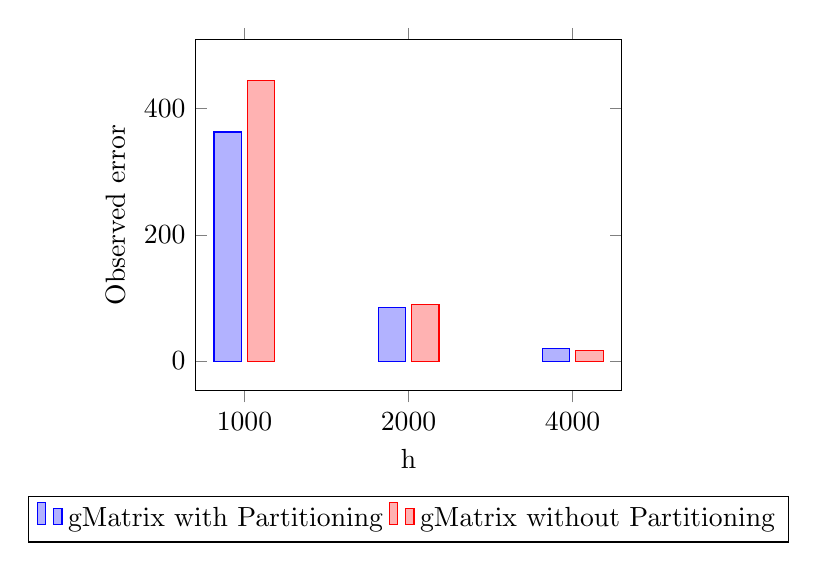
\begin{tikzpicture}
  \begin{axis}[
      ybar,
      enlargelimits=0.15,
      legend style={at={(0.5,-0.3)},anchor=north,legend columns=-1},
      ylabel={Observed error},
      xlabel={h},
      width=7cm,
      symbolic x coords={1000,2000,4000},
      xtick=data
    ]
      \addplot 
	  coordinates {
        (1000,  362.84)
        (2000,  85.24)
        (4000,  19.31)
      };
      \addplot 
	  coordinates {
        (1000,  444.81)
        (2000,  90.16)
        (4000,  17.30)
      };
      \legend{gMatrix with Partitioning,gMatrix without Partitioning}
  \end{axis}
\end{tikzpicture}
\caption{Observed error on Friendster dataset considered over 1 million random edges} \label{fig:F11}
\end{figure}

\begin{figure}[!htbp]
\centering
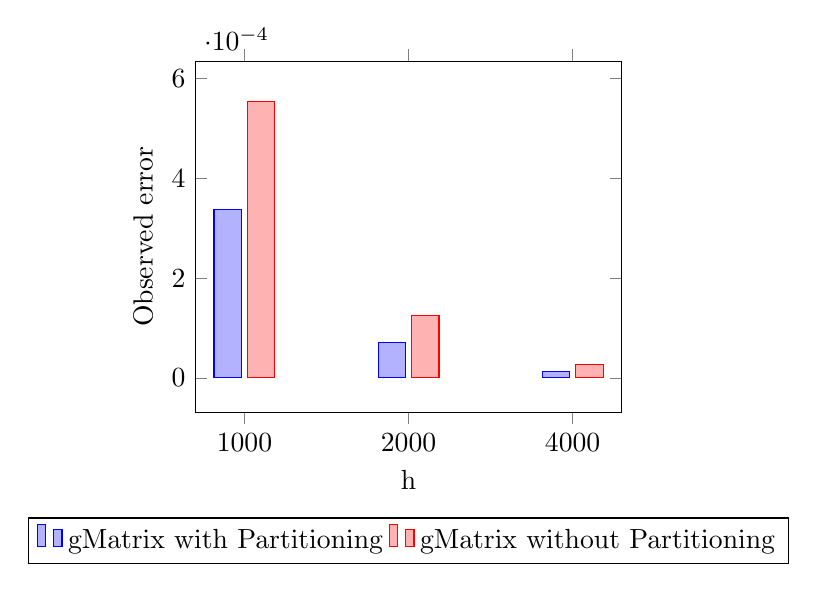
\begin{tikzpicture}
  \begin{axis}[
      ybar,
      enlargelimits=0.15,
      legend style={at={(0.5,-0.3)},anchor=north,legend columns=-1},
      ylabel={Observed error},
      xlabel={h},
      width=7cm,
      symbolic x coords={1000,2000,4000},
      xtick=data
    ]
      \addplot 
	  coordinates {
        (1000,  0.000338304)
        (2000,  7.17931e-05)
        (4000,  1.25923e-05)
      };
      \addplot 
	  coordinates {
        (1000,  0.000553365)
        (2000,  0.000124219)
        (4000,  2.61629e-05)
      };
      \legend{gMatrix with Partitioning, gMatrix without Partitioning}
  \end{axis}
\end{tikzpicture}
\caption{Observed error on Friendster dataset considered over top-500 highest frequency edges} \label{fig:F12}
\end{figure}

% Average relative error

\begin{figure}[!htbp]
\centering
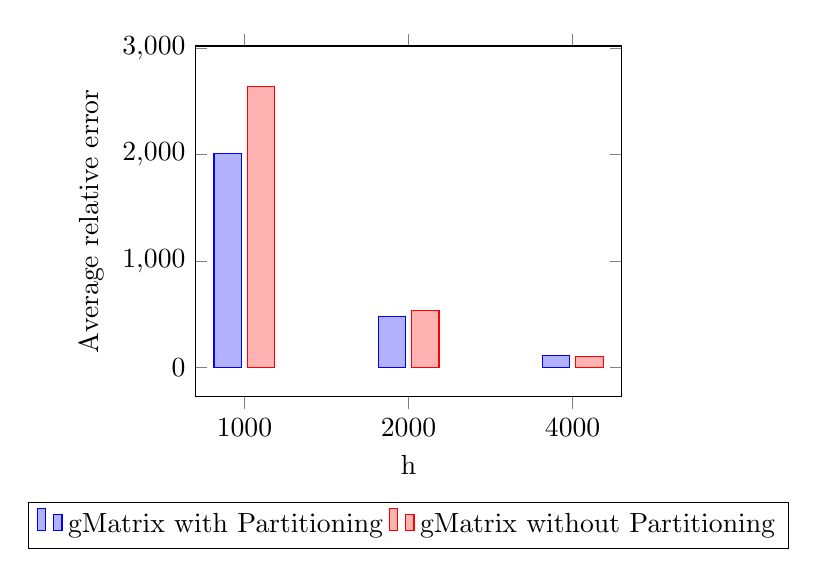
\begin{tikzpicture}
  \begin{axis}[
      ybar,
      enlargelimits=0.15,
      legend style={at={(0.5,-0.3)},anchor=north,legend columns=-1},
      ylabel={Average relative error},
      xlabel={h},
      width=7cm,
      symbolic x coords={1000,2000,4000},
      xtick=data
    ]
      \addplot 
	  coordinates {
        (1000,  2009.98)
        (2000,  478.512)
        (4000,  110.623)
      };
      \addplot 
	  coordinates {
        (1000,  2642.89)
        (2000,  535.386)
        (4000,  102.601)
      };
      \legend{gMatrix with Partitioning,gMatrix without Partitioning}
  \end{axis}
\end{tikzpicture}
\caption{Average relative error on Friendster dataset considered over 1 million random edges} \label{fig:F21}
\end{figure}

\begin{figure}[!htbp]
\centering
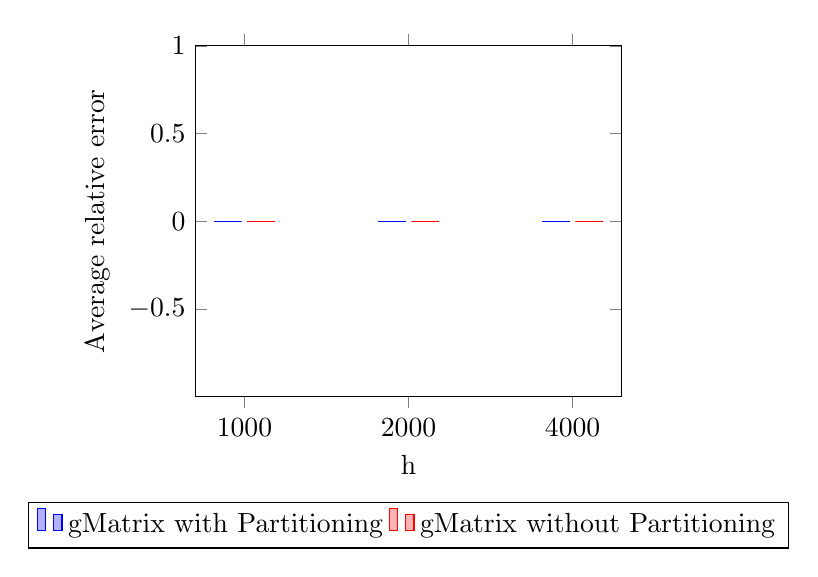
\begin{tikzpicture}
  \begin{axis}[
      ybar,
      enlargelimits=0.15,
      legend style={at={(0.5,-0.3)},anchor=north,legend columns=-1},
      ylabel={Average relative error},
      xlabel={h},
      width=7cm,
      symbolic x coords={1000,2000,4000},
      xtick=data
    ]
      \addplot 
	  coordinates {
        (1000,  0)
        (2000,  0)
        (4000,  0)
      };
      \addplot 
	  coordinates {
        (1000,  0)
        (2000,  0)
        (4000,  0)
      };
      \legend{gMatrix with Partitioning, gMatrix without Partitioning}
  \end{axis}
\end{tikzpicture}
\caption{Average relative error on Friendster dataset considered over top-500 highest frequency edges} \label{fig:F22}
\end{figure}

% Effective queries

\begin{figure}[!htbp]
\centering
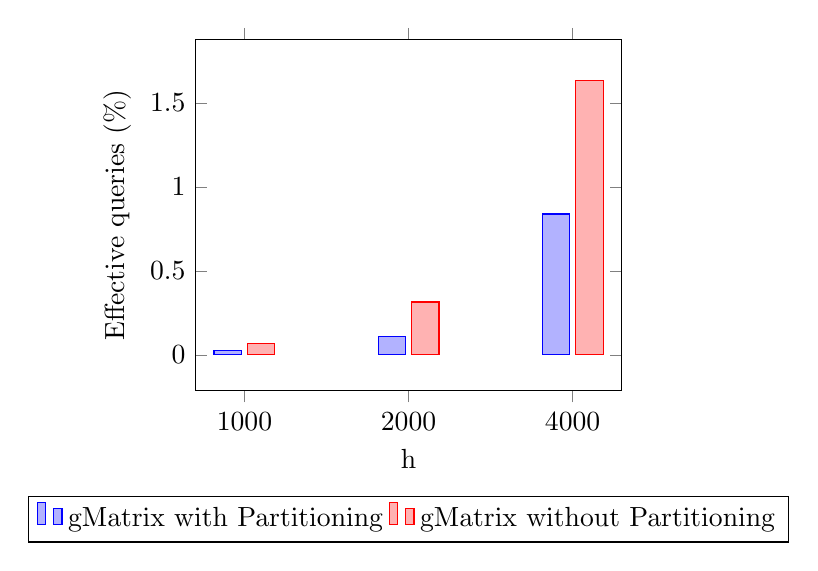
\begin{tikzpicture}
  \begin{axis}[
      ybar,
      enlargelimits=0.15,
      legend style={at={(0.5,-0.3)},anchor=north,legend columns=-1},
      ylabel={Effective queries (\%)},
      xlabel={h},
      width=7cm,
      symbolic x coords={1000,2000,4000},
      xtick=data
    ]
      \addplot 
	  coordinates {
        (1000,  0.0285)
        (2000,  0.1098)
        (4000,  0.8383)
      };
      \addplot 
	  coordinates {
        (1000,  0.0671)
        (2000,  0.3152)
        (4000,  1.6345)
      };
      \legend{gMatrix with Partitioning,gMatrix without Partitioning}
  \end{axis}
\end{tikzpicture}
\caption{Effective queries percentage on Friendster dataset considered over 1 million random edges} \label{fig:F31}
\end{figure}

\begin{figure}[!htbp]
\centering
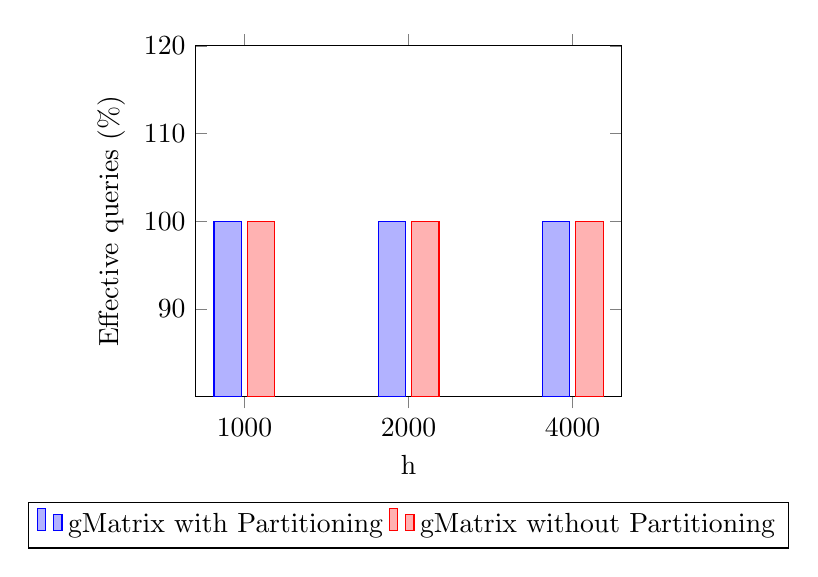
\begin{tikzpicture}
  \begin{axis}[
      ybar,
      enlargelimits=0.15,
      legend style={at={(0.5,-0.3)},anchor=north,legend columns=-1},
      ylabel={Effective queries (\%)},
      xlabel={h},
      width=7cm,
      symbolic x coords={1000,2000,4000},
      xtick=data
    ]
      \addplot 
	  coordinates {
        (1000,  100)
        (2000,  100)
        (4000,  100)
      };
      \addplot 
	  coordinates {
        (1000,  100)
        (2000,  100)
        (4000,  100)
      };
      \legend{gMatrix with Partitioning, gMatrix without Partitioning}
  \end{axis}
\end{tikzpicture}
\caption{Effective queries percentage on Friendster dataset considered over top-500 highest frequency edges} \label{fig:F32}
\end{figure}

\paragraph{Friendster dataset}
Partitioning reduces the observed error and the average relative error of the estimations, as seen on figures \ref{fig:F11}-\ref{fig:F21}. The lower errors are possible because partitioning reduces the number of queries with high relative errors (queries $q$ such that $\frac{\tilde{f}(q)-f(q)}{f(q)} > T$), as the number of effective queries themselves are actually lower with partitioning as seen on figure \ref{fig:F31}.

%Twitter
%Observed error
\clearpage

\begin{figure}[!htbp]
\centering
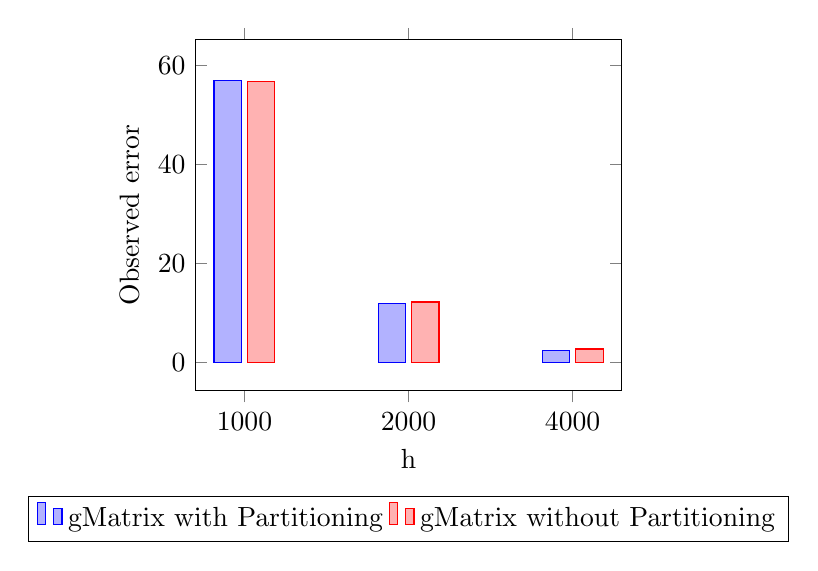
\begin{tikzpicture}
  \begin{axis}[
      ybar,
      enlargelimits=0.15,
      legend style={at={(0.5,-0.3)},anchor=north,legend columns=-1},
      ylabel={Observed error},
      xlabel={h},
      width=7cm,
      symbolic x coords={1000,2000,4000},
      xtick=data
    ]
      \addplot 
	  coordinates {
        (1000,  56.9662)
        (2000,  11.94)
        (4000,  2.4375)
      };
      \addplot 
	  coordinates {
        (1000,  56.7384)
        (2000,  12.1534)
        (4000,  2.67581)
      };
      \legend{gMatrix with Partitioning,gMatrix without Partitioning}
  \end{axis}
\end{tikzpicture}
\caption{Observed error of Twitter dataset considered over 1 million random edges} \label{fig:T11}
\end{figure}

\begin{figure}[!htbp]
\centering
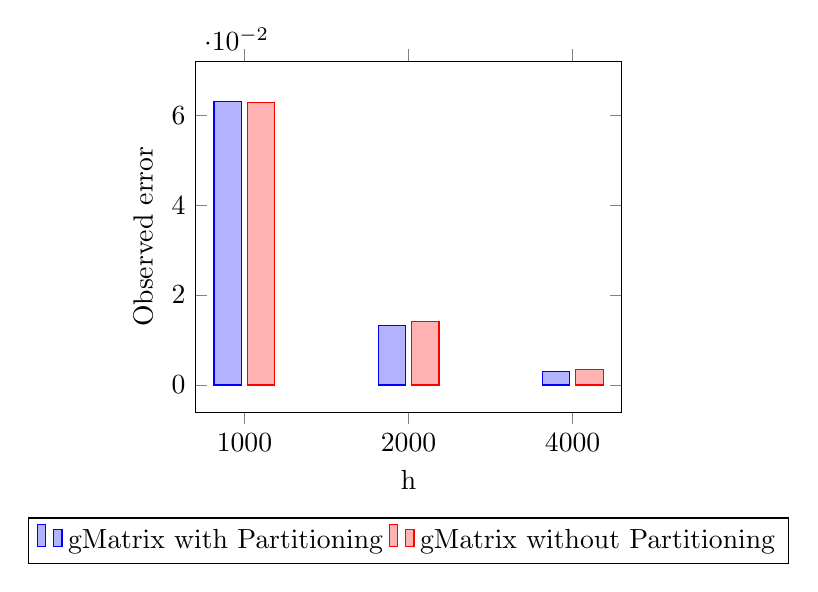
\begin{tikzpicture}
  \begin{axis}[
      ybar,
      enlargelimits=0.15,
      legend style={at={(0.5,-0.3)},anchor=north,legend columns=-1},
      ylabel={Observed error},
      xlabel={h},
      width=7cm,
      symbolic x coords={1000,2000,4000},
      xtick=data
    ]
      \addplot 
	  coordinates {
        (1000,  0.0630049)
        (2000,  0.0132349)
        (4000,  0.00296191)
      };
      \addplot 
	  coordinates {
        (1000,  0.0628949)
        (2000,  0.0140856)
        (4000,  0.00347708)
      };
      \legend{gMatrix with Partitioning, gMatrix without Partitioning}
  \end{axis}
\end{tikzpicture}
\caption{Observed error of Twitter dataset considered over top-500 highest frequency edges} \label{fig:T12}
\end{figure}

% Average relative error

\begin{figure}[!htbp]
\centering
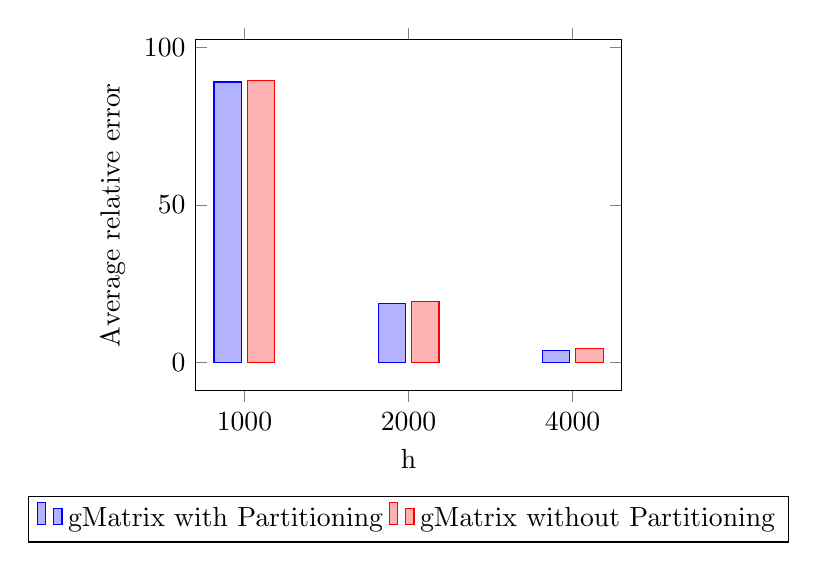
\begin{tikzpicture}
  \begin{axis}[
      ybar,
      enlargelimits=0.15,
      legend style={at={(0.5,-0.3)},anchor=north,legend columns=-1},
      ylabel={Average relative error},
      xlabel={h},
      width=7cm,
      symbolic x coords={1000,2000,4000},
      xtick=data
    ]
      \addplot 
	  coordinates {
        (1000,  88.956)
        (2000,  18.7822)
        (4000,  3.89071)
      };
      \addplot 
	  coordinates {
        (1000,  89.5238)
        (2000,  19.2599)
        (4000,  4.27863)
      };
      \legend{gMatrix with Partitioning,gMatrix without Partitioning}
  \end{axis}
\end{tikzpicture}
\caption{Average relative error on Twitter dataset considered over 1 million random edges} \label{fig:T21}
\end{figure}

\begin{figure}[!htbp]
\centering
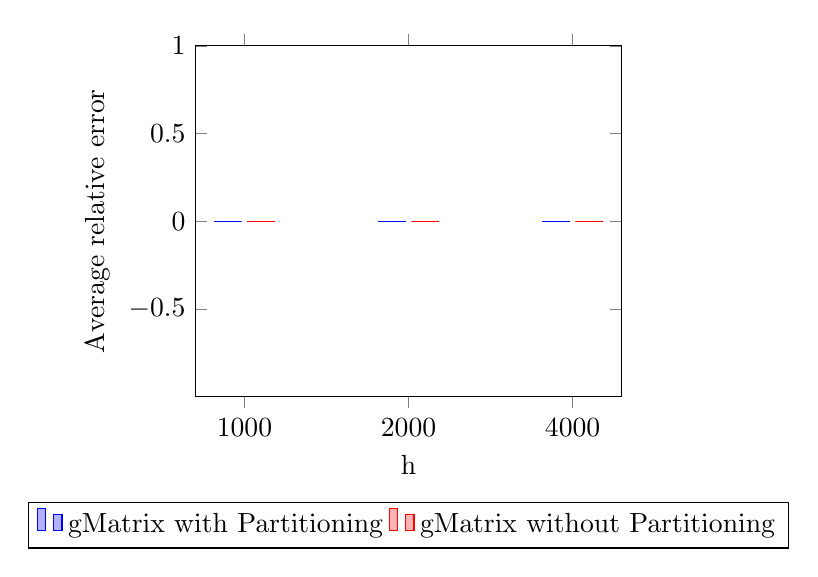
\begin{tikzpicture}
  \begin{axis}[
      ybar,
      enlargelimits=0.15,
      legend style={at={(0.5,-0.3)},anchor=north,legend columns=-1},
      ylabel={Average relative error},
      xlabel={h},
      width=7cm,
      symbolic x coords={1000,2000,4000},
      xtick=data
    ]
      \addplot 
	  coordinates {
        (1000,  0)
        (2000,  0)
        (4000,  0)
      };
      \addplot 
	  coordinates {
        (1000,  0)
        (2000,  0)
        (4000,  0)
      };
      \legend{gMatrix with Partitioning, gMatrix without Partitioning}
  \end{axis}
\end{tikzpicture}
\caption{Average relative error on Twitter dataset considered over top-500 highest frequency edges} \label{fig:T22}
\end{figure}

% Effective queries

\begin{figure}[!htbp]
\centering
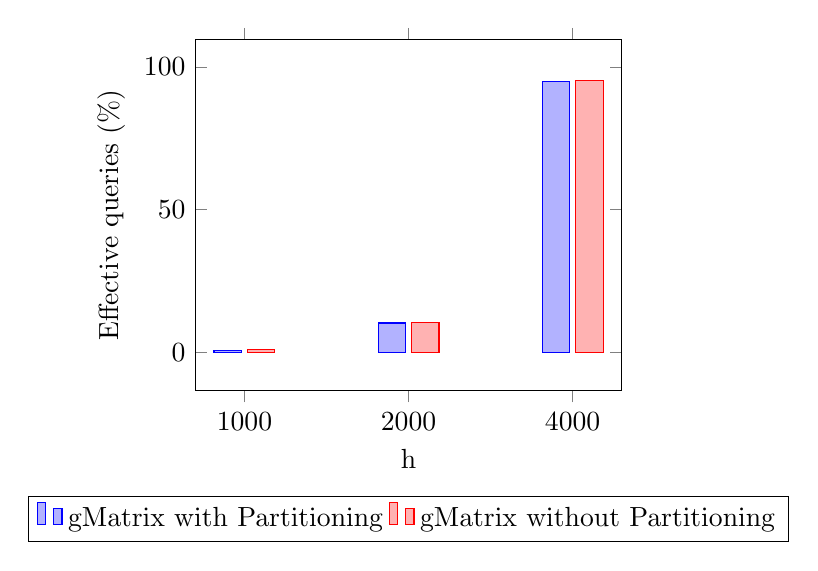
\begin{tikzpicture}
  \begin{axis}[
      ybar,
      enlargelimits=0.15,
      legend style={at={(0.5,-0.3)},anchor=north,legend columns=-1},
      ylabel={Effective queries (\%)},
      xlabel={h},
      width=7cm,
      symbolic x coords={1000,2000,4000},
      xtick=data
    ]
      \addplot 
	  coordinates {
        (1000,  0.6977)
        (2000,  10.214)
        (4000,  94.9675)
      };
      \addplot 
	  coordinates {
        (1000,  0.8046)
        (2000,  10.4912)
        (4000,  95.3025)
      };
      \legend{gMatrix with Partitioning,gMatrix without Partitioning}
  \end{axis}
\end{tikzpicture}
\caption{Effective queries percentage on Twitter dataset considered over 1 million random edges} \label{fig:T31}
\end{figure}

\begin{figure}[!htbp]
\centering
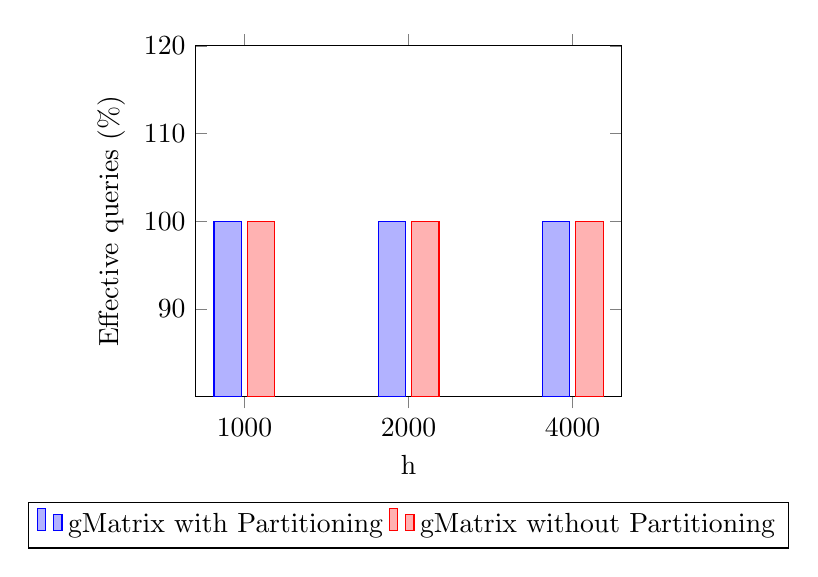
\begin{tikzpicture}
  \begin{axis}[
      ybar,
      enlargelimits=0.15,
      legend style={at={(0.5,-0.3)},anchor=north,legend columns=-1},
      ylabel={Effective queries (\%)},
      xlabel={h},
      width=7cm,
      symbolic x coords={1000,2000,4000},
      xtick=data
    ]
      \addplot 
	  coordinates {
        (1000,  100)
        (2000,  100)
        (4000,  100)
      };
      \addplot 
	  coordinates {
        (1000,  100)
        (2000,  100)
        (4000,  100)
      };
      \legend{gMatrix with Partitioning, gMatrix without Partitioning}
  \end{axis}
\end{tikzpicture}
\caption{Effective queries percentage on Twitter dataset considered over top-500 highest frequency edges} \label{fig:T32}
\end{figure}

\paragraph{Twitter dataset}
Partitioning does not seem to be effective at all as seen on figures \ref{fig:T11}-\ref{fig:T32}.


%IP Trace
%Observed error
\clearpage
\begin{figure}[!htbp]
\centering
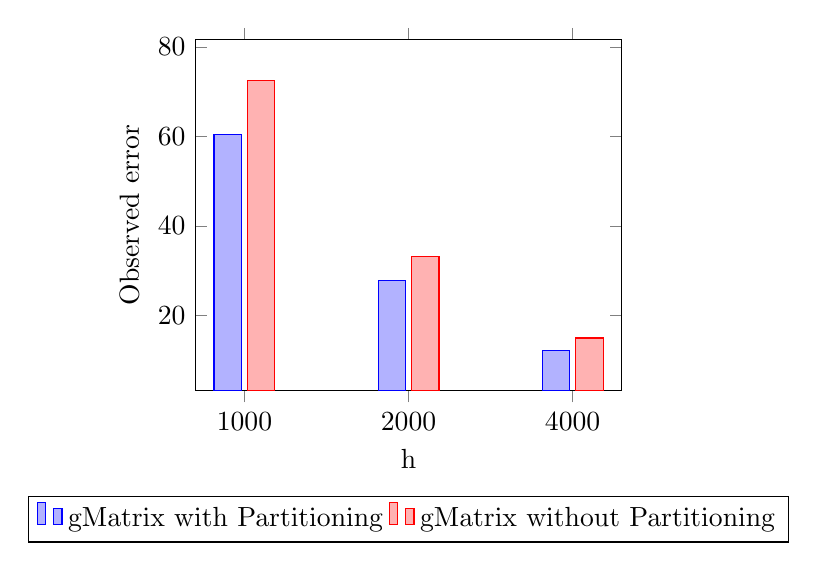
\begin{tikzpicture}
  \begin{axis}[
      ybar,
      enlargelimits=0.15,
      legend style={at={(0.5,-0.3)},anchor=north,legend columns=-1},
      ylabel={Observed error},
      xlabel={h},
      width=7cm,
      symbolic x coords={1000,2000,4000},
      xtick=data
    ]
      \addplot 
	  coordinates {
        (1000,  60.3821)
        (2000,  27.8266)
        (4000,  12.2106)
      };
      \addplot 
	  coordinates {
        (1000,  72.5277)
        (2000,  33.2313)
        (4000,  14.9191)
      };
      \legend{gMatrix with Partitioning,gMatrix without Partitioning}
  \end{axis}
\end{tikzpicture}
\caption{Observed error of IP-Trace dataset considered over 1 million random edges} \label{fig:I11}
\end{figure}

\begin{figure}[!htbp]
\centering
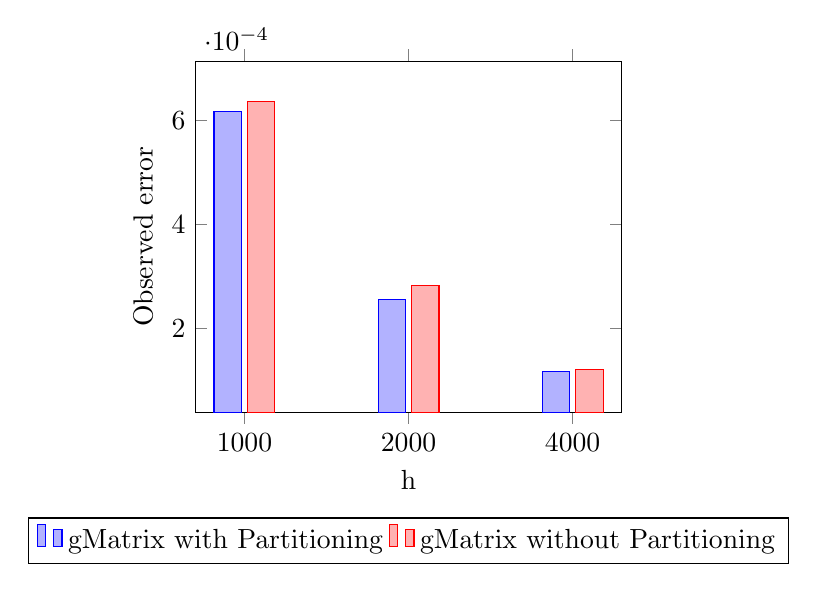
\begin{tikzpicture}
  \begin{axis}[
      ybar,
      enlargelimits=0.15,
      legend style={at={(0.5,-0.3)},anchor=north,legend columns=-1},
      ylabel={Observed error},
      xlabel={h},
      width=7cm,
      symbolic x coords={1000,2000,4000},
      xtick=data
    ]
      \addplot 
	  coordinates {
        (1000,  0.000616909)
        (2000,  0.000255977)
        (4000,  0.000116424)
      };
      \addplot 
	  coordinates {
        (1000,  0.000635283)
        (2000,  0.000282608)
        (4000,  0.000120565)
      };
      \legend{gMatrix with Partitioning, gMatrix without Partitioning}
  \end{axis}
\end{tikzpicture}
\caption{Observed error of IP-Trace dataset considered over top-500 highest frequency edges} \label{fig:I12}
\end{figure}

% Average relative error

\begin{figure}[!htbp]
\centering
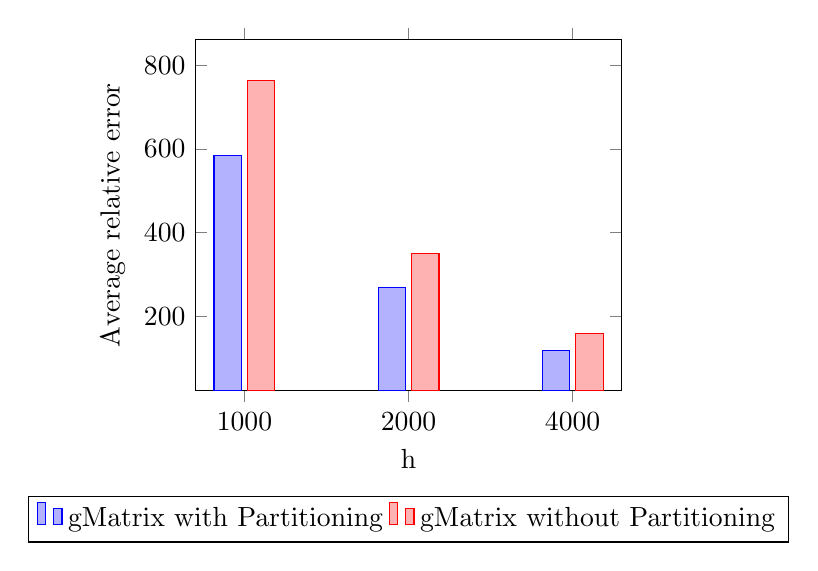
\begin{tikzpicture}
  \begin{axis}[
      ybar,
      enlargelimits=0.15,
      legend style={at={(0.5,-0.3)},anchor=north,legend columns=-1},
      ylabel={Average relative error},
      xlabel={h},
      width=7cm,
      symbolic x coords={1000,2000,4000},
      xtick=data
    ]
      \addplot 
	  coordinates {
        (1000,  583.576)
        (2000,  268.387)
        (4000,  118.987)
      };
      \addplot 
	  coordinates {
        (1000,  764.424)
        (2000,  350.601)
        (4000,  157.765)
      };
      \legend{gMatrix with Partitioning,gMatrix without Partitioning}
  \end{axis}
\end{tikzpicture}
\caption{Average relative error on IP-Trace dataset considered over 1 million random edges} \label{fig:I21}
\end{figure}

\begin{figure}[!htbp]
\centering
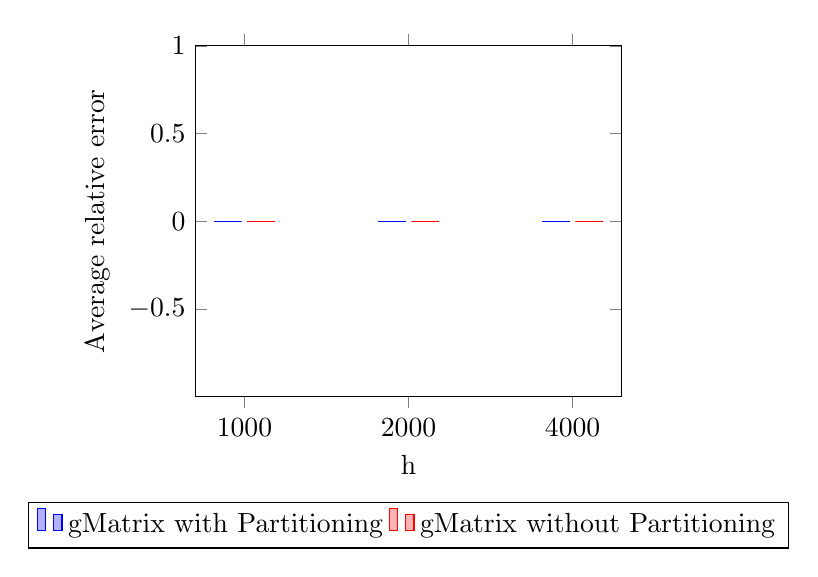
\begin{tikzpicture}
  \begin{axis}[
      ybar,
      enlargelimits=0.15,
      legend style={at={(0.5,-0.3)},anchor=north,legend columns=-1},
      ylabel={Average relative error},
      xlabel={h},
      width=7cm,
      symbolic x coords={1000,2000,4000},
      xtick=data
    ]
      \addplot 
	  coordinates {
        (1000,  0)
        (2000,  0)
        (4000,  0)
      };
      \addplot 
	  coordinates {
        (1000,  0)
        (2000,  0)
        (4000,  0)
      };
      \legend{gMatrix with Partitioning, gMatrix without Partitioning}
  \end{axis}
\end{tikzpicture}
\caption{Average relative error on IP-Trace dataset considered over top-500 highest frequency edges} \label{fig:I22}
\end{figure}

% Effective queries

\begin{figure}[!htbp]
\centering
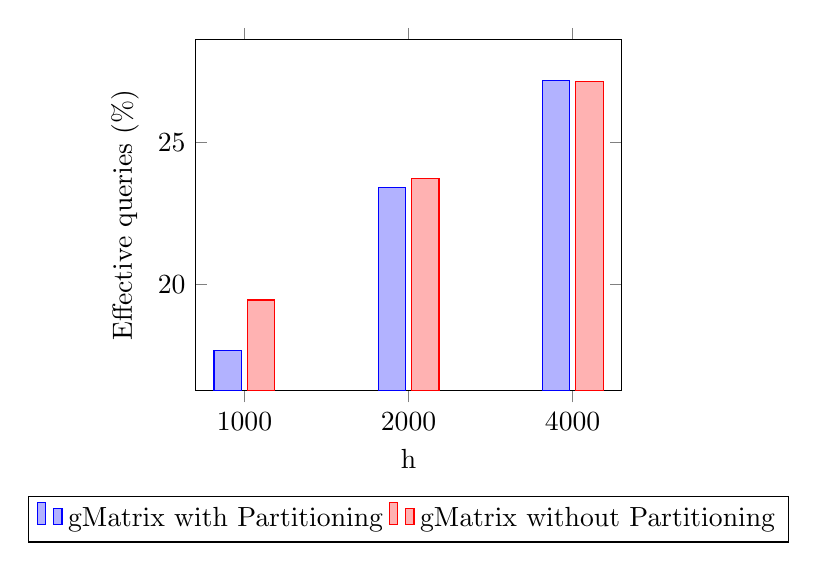
\begin{tikzpicture}
  \begin{axis}[
      ybar,
      enlargelimits=0.15,
      legend style={at={(0.5,-0.3)},anchor=north,legend columns=-1},
      ylabel={Effective queries (\%)},
      xlabel={h},
      width=7cm,
      symbolic x coords={1000,2000,4000},
      xtick=data
    ]
      \addplot 
	  coordinates {
        (1000,  17.6949)
        (2000,  23.426)
        (4000,  27.1898)
      };
      \addplot 
	  coordinates {
        (1000,  19.4597)
        (2000,  23.7307)
        (4000,  27.16)
      };
      \legend{gMatrix with Partitioning,gMatrix without Partitioning}
  \end{axis}
\end{tikzpicture}
\caption{Effective queries percentage on IP-Trace dataset considered over 1 million random edges} \label{fig:I31}
\end{figure}

\begin{figure}[!htbp]
\centering
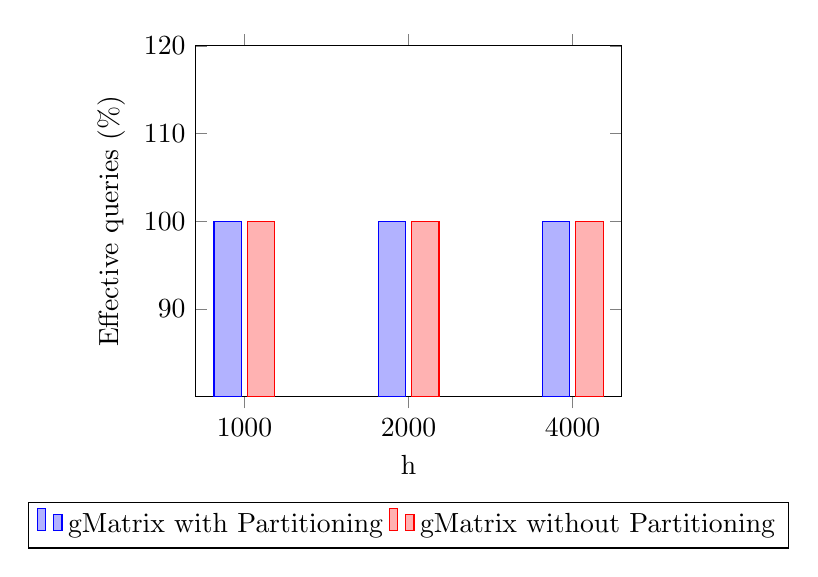
\begin{tikzpicture}
  \begin{axis}[
      ybar,
      enlargelimits=0.15,
      legend style={at={(0.5,-0.3)},anchor=north,legend columns=-1},
      ylabel={Effective queries (\%)},
      xlabel={h},
      width=7cm,
      symbolic x coords={1000,2000,4000},
      xtick=data
    ]
      \addplot 
	  coordinates {
        (1000,  100)
        (2000,  100)
        (4000,  100)
      };
      \addplot 
	  coordinates {
        (1000,  100)
        (2000,  100)
        (4000,  100)
      };
      \legend{gMatrix with Partitioning, gMatrix without Partitioning}
  \end{axis}
\end{tikzpicture}
\caption{Effective queries percentage on IP-Trace dataset considered over top-500 highest frequency edges} \label{fig:I32}
\end{figure}

\paragraph{IP-Trace dataset}
Partitioning reduces the observed error and the average relative error of the estimations, as seen on figures \ref{fig:I11}-\ref{fig:I21}. Unlike the results on the Friendster dataset, the number of effective queries after partitioning are only significantly lower on $h=1000$ and is actually higher than without partitioning on $h=4000$.

% Heavy hitter
\clearpage
\subsection{Heavy Hitter Edge Estimation}

\begin{figure}[!htbp]
\centering
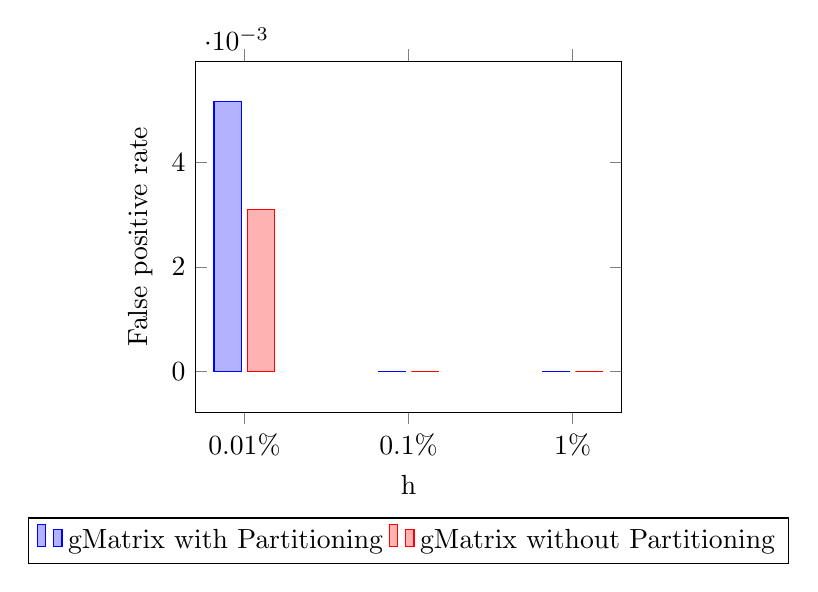
\begin{tikzpicture}
  \begin{axis}[
      ybar,
      enlargelimits=0.15,
      legend style={at={(0.5,-0.3)},anchor=north,legend columns=-1},
      ylabel={False positive rate},
      xlabel={h},
      width=7cm,
      symbolic x coords={0.01\%,0.1\%,1\%},
      xtick=data
    ]
      \addplot 
	  coordinates {
        (0.01\%,0.00515996)
        (0.1\%, 0)
        (1\%,   0)
      };
      \addplot 
	  coordinates {
        (0.01\%,  0.00309598)
        (0.1\%,   0)
        (1\%,     0)
      };
      \legend{gMatrix with Partitioning, gMatrix without Partitioning}
  \end{axis}
\end{tikzpicture}
\caption{False positive rate of heavy hitter edge estimation on IP-Trace dataset} \label{fig:EE1}
\end{figure}

\begin{figure}[!htbp]
\centering
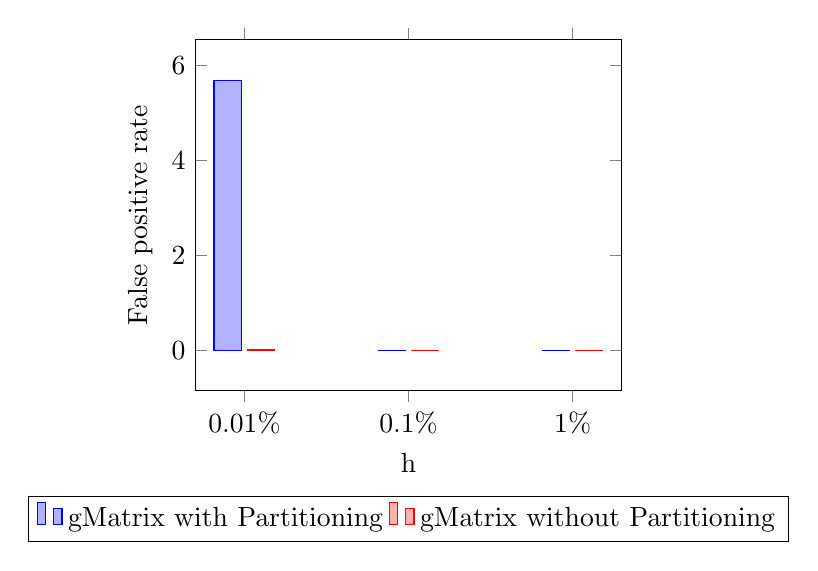
\begin{tikzpicture}
  \begin{axis}[
      ybar,
      enlargelimits=0.15,
      legend style={at={(0.5,-0.3)},anchor=north,legend columns=-1},
      ylabel={False positive rate},
      xlabel={h},
      width=7cm,
      symbolic x coords={0.01\%,0.1\%,1\%},
      xtick=data
    ]
      \addplot 
	  coordinates {
        (0.01\%,5.691796)
        (0.1\%, 0)
        (1\%,   0)
      };
      \addplot 
	  coordinates {
        (0.01\%,  0.015521)
        (0.1\%,   0)
        (1\%,     0)
      };
      \legend{gMatrix with Partitioning, gMatrix without Partitioning}
  \end{axis}
\end{tikzpicture}
\caption{False positive rate of heavy hitter edge estimation on Friendster dataset} \label{fig:EE2}
\end{figure}
